\subsection{Herstellung der Compact Disc mittels des Spritzgussverfahrens}
\label{subsec:cdherstellung}

Die Herstellung einer vorbespielten CD beginnt mit der in
\autoref{fig:cdherstellung} dargestellten Anfertigung einer Metallmatrize für
das Spritzgussverfahren. Dafür wird eine Glasplatte mit Fotolack beschichtet.
Mittels Belichtung wird das \textit{pit}-Muster der CD auf die Fotolackschicht
übertragen. Nach dem Entfernen des belichteten Fotolacks wird ein Negativ der
Glasmatrize in Form einer Metallmatrize erstellt. Durch das Spritzgussverfahren
wird das \textit{pit}-Muster von der Metallmatrize auf die Polycarbonatscheibe
übertragen. Um eine Reflexionsschicht zu erhalten, wird auf das Polycarbonat
Aluminium aufgedampft. Im letzten Schritt wird die Reflexionsschicht mit einer
Schutzschicht versiegelt. \cite{cdp}

\ifthenelse{\boolean{showPics}}{
    \begin{figure}[h]
        \begin{center}
            \begin{minipage}[t]{\textwidth}
                \begin{center}
                    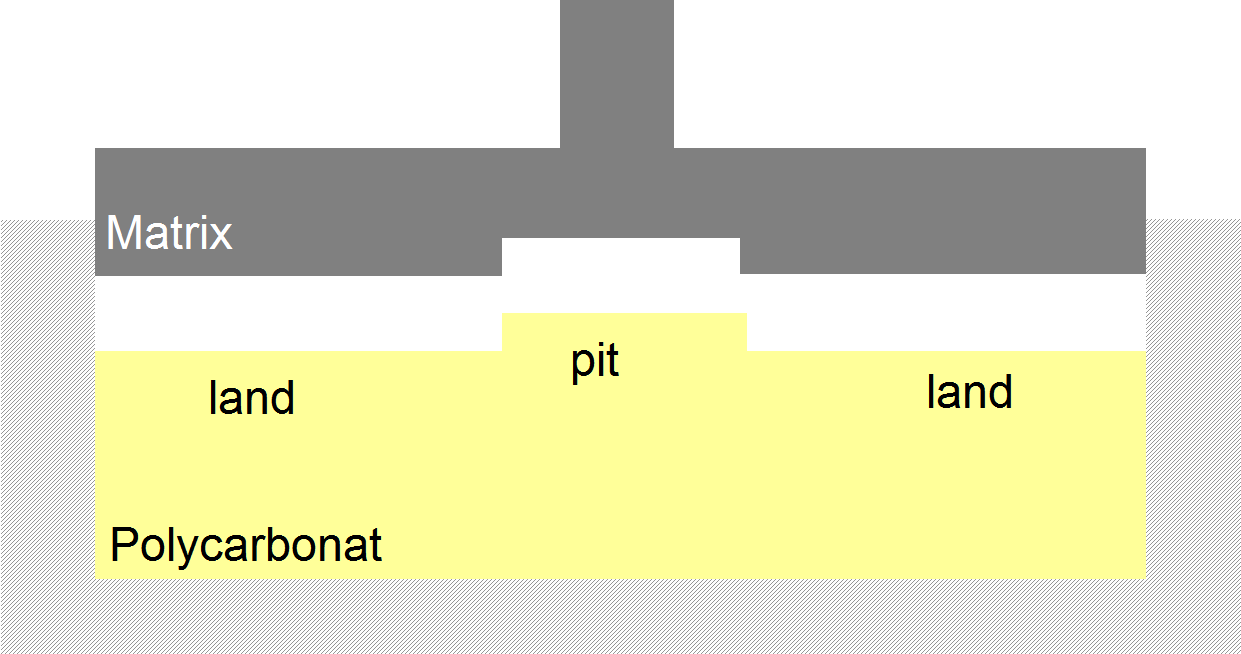
\includegraphics[width=\textwidth]{Bilder/Optische_Datentraeger_Die_Compact_Disc/Herstellung/cdherstellung.png}
                    \caption[Herstellung der Metallmatrize und der CD \newline basierend auf \url{http://www.muenster.de/~asshoff/physik/cd/image46.gif} (zuletzt aufgerufen am 01.11.2015)]{Herstellung der Metallmatrize und der CD}
                    \label{fig:cdherstellung}
                \end{center}
            \end{minipage}
        \end{center}
    \end{figure}
}{}

Das Spritzgussverfahren selbst unterteilt sich in drei Schritte. Wie in
\autoref{fig:cdspritz} dargestellt, wird zunächst zerkleinertes Polycarbonat
(Granulat) in die Schnecke eingefüllt. Durch die Heizelemente verflüssigt sich
das Granulat und die sich drehende Schnecke befördert es an die Spitze des
Plastifizierzylinders. Dieser Schritt heißt Plastifizieren.
Der sich an der Spitze des Plastifizierzylinders aufbauende Druck presst die
Schnecke teilweise aus dem Zylinder. Danach folgt der Einspritzvorgang. Dabei
wird das geschmolzene Granulat durch die Vorwärtsbewegung der Schnecke in die
CD-Form und auf die Metallmatrize gedrückt. Nach dem Abkühlen wird die fertige
Polycarbonatscheibe ausgeworfen. \cite{cdpf}

\ifthenelse{\boolean{showPics}}{
    \begin{figure}[h]
        \begin{center}
            \begin{minipage}[t]{\textwidth}
                \begin{center}
                    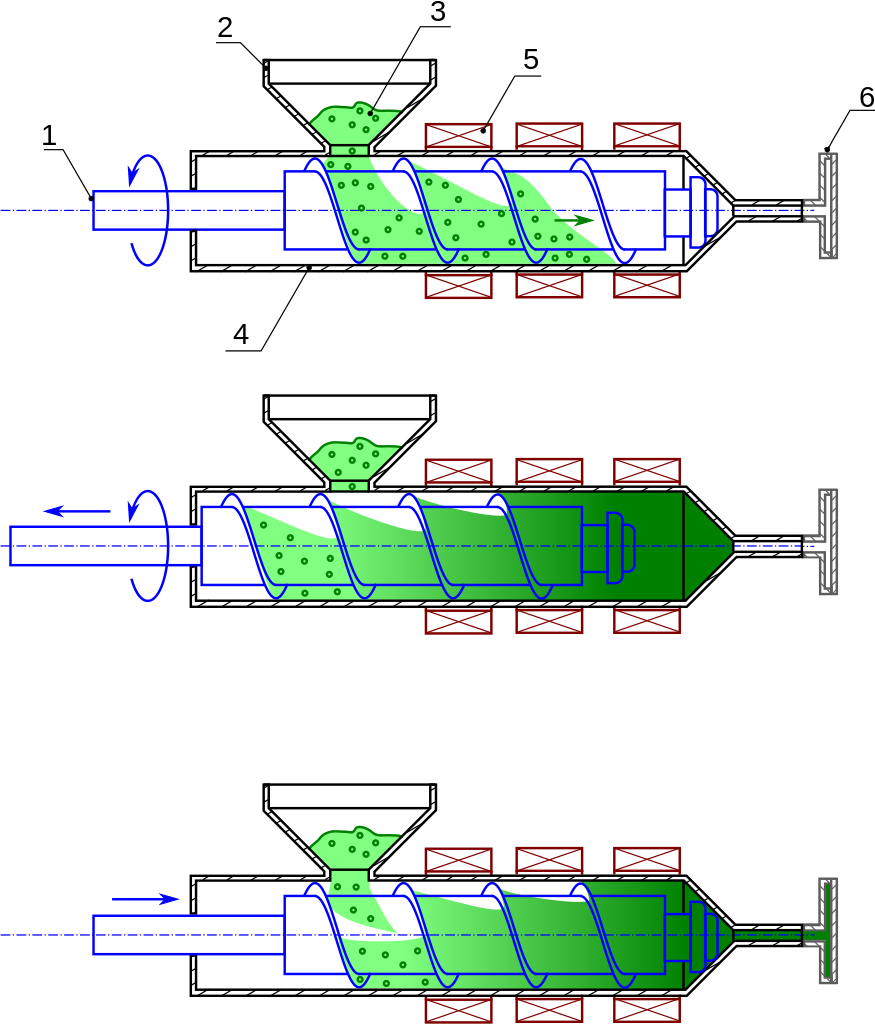
\includegraphics[height=0.5\textheight]{Bilder/Optische_Datentraeger_Die_Compact_Disc/Herstellung/cdspritz.png}
                    \caption[Spritzgussverfahren \newline \url{https://upload.wikimedia.org/wikipedia/commons/thumb/2/23/Principe_moulage_injection_polymere.svg/899px-Principe_moulage_injection_polymere.svg.png} (zuletzt aufgerufen am 11.08.2015)]{Spritzgussverfahren: 1. Schnecke, 2. Einfülltrichter, 3. Granulat, 4. Plastifizier\-zylinder, 5. Heizelemente, 6. CD-Form inklusive Metallmatrize}
                    \label{fig:cdspritz}
                \end{center}
            \end{minipage}
        \end{center}
    \end{figure}
}{}

\newpage
